\subsubsection{Organigrama y Descripción de Roles - ¿Quién se ocupa de cada responsabilidad?}\label{sec:spmp-8-4-2}
El equipo está conformado por Andrés Felipe Pinzón Márquez, Daniel Felipe Ramírez Vargas, Guillermo Andrés Aponte Cárdenas y Miguel Ángel Sarmiento Cuervo. Adopta los roles de DAD descritos en la tabla~\ref{tab:roles}, conservando sus nombres en inglés~\cite{ambler2012dad,pmiDADroles}. Todos actúan como \textit{Team Members}: analizan, diseñan, desarrollan, prueban, documentan, estiman y reportan sus tareas. Los roles de coordinación añaden responsabilidades específicas, sin establecer una división permanente por especialidades.

\begin{figure}[!htbp]
\centering
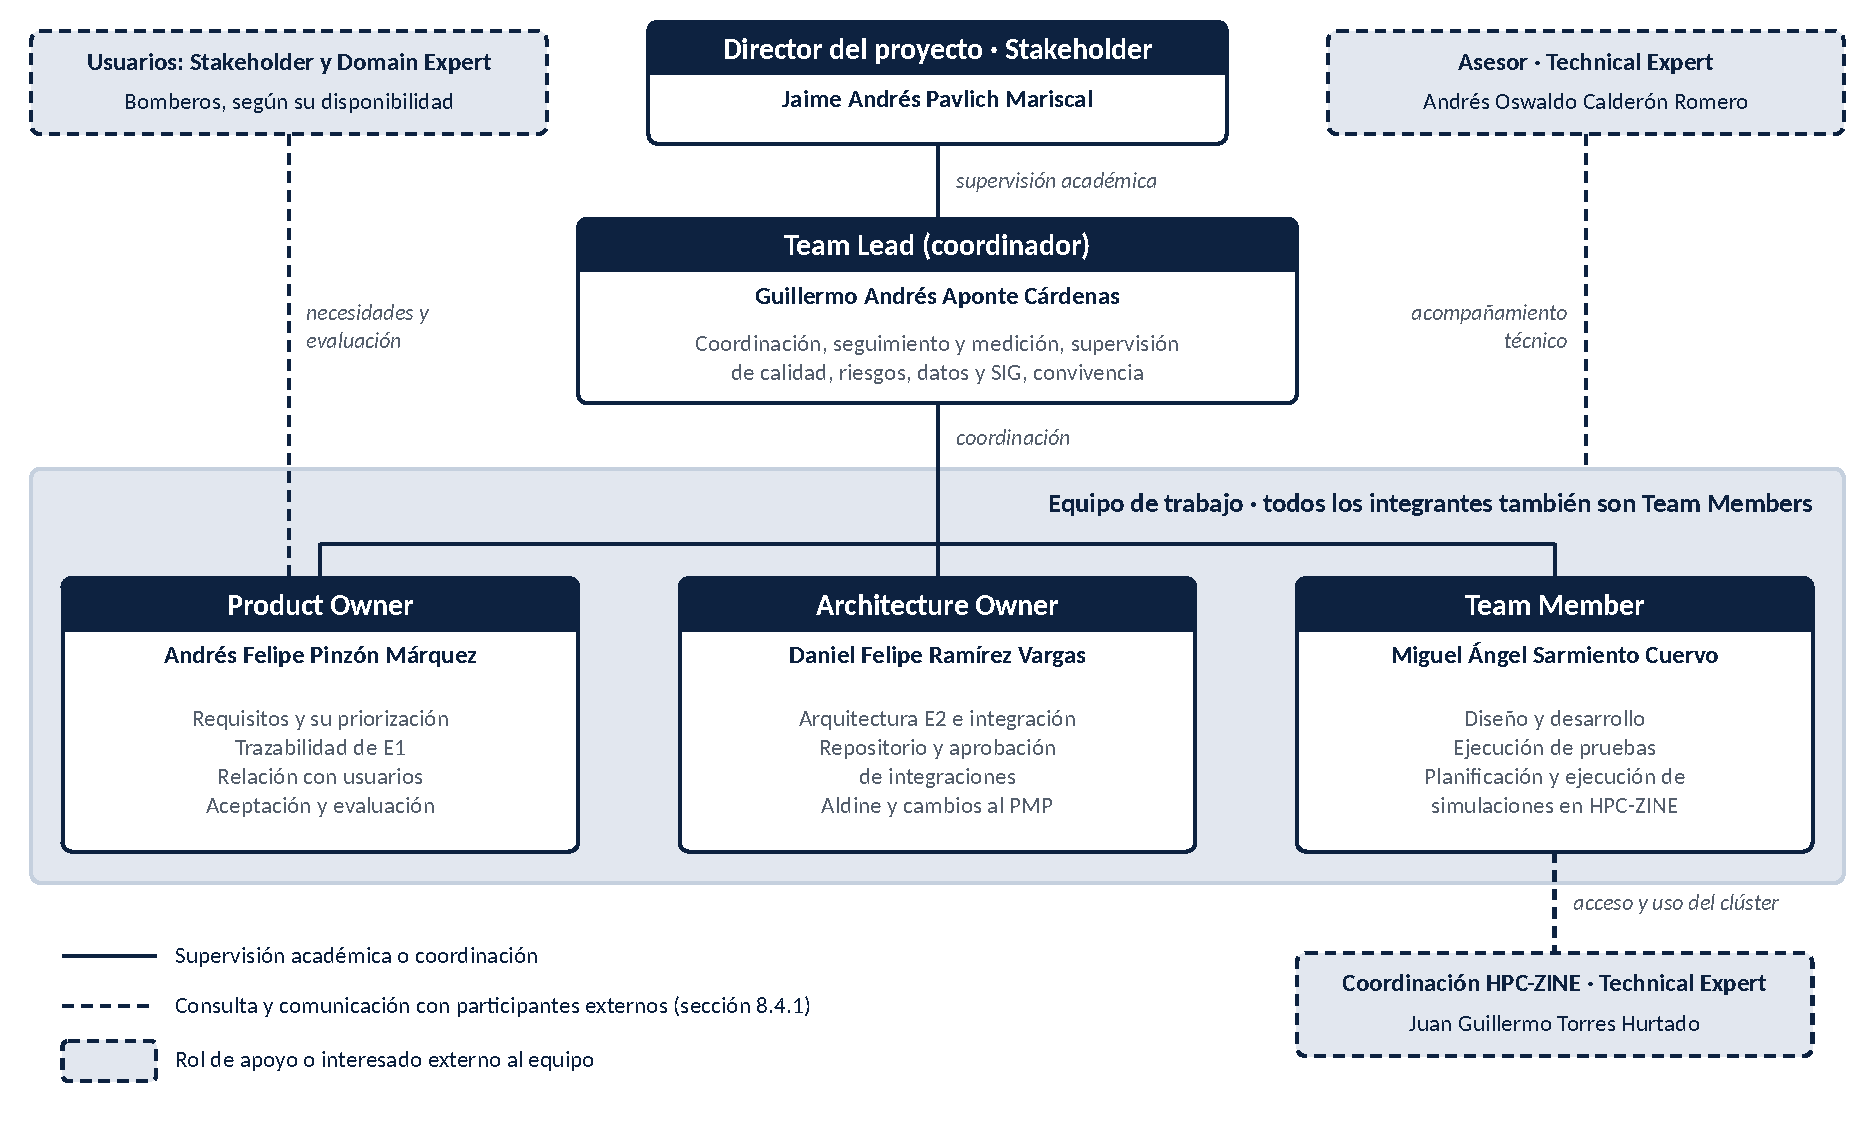
\includegraphics[width=\linewidth,height=0.35\textheight,keepaspectratio]{organigrama.pdf}
\caption{Organigrama del proyecto. Fuente: elaboración propia a partir de los roles de DAD~\cite{ambler2012dad}.}
\label{fig:organigrama}
\end{figure}

La figura~\ref{fig:organigrama} distingue la supervisión académica del director y la coordinación interna. El \textit{Team Lead} facilita el trabajo y remueve impedimentos, sin autoridad de mando. El \textit{Product Owner} orienta las prioridades y el \textit{Architecture Owner}, las decisiones técnicas; sus propuestas se acuerdan mediante las reglas de la sección~12.1. Los cambios al plan requieren la aprobación del director y de todos los integrantes (sección~6.6). Las líneas punteadas indican consulta con los participantes externos de la sección~8.4.1, sin subordinación jerárquica.

\paragraph{Roles y responsabilidades.} La asignación se apoya en las fortalezas del equipo: comunicación y resolución de problemas de Guillermo; capacidad técnica y experiencia en control de versiones de Daniel; relación con los interesados de Andrés, y dedicación al desarrollo, las pruebas y las simulaciones de Miguel. En la tabla~\ref{tab:roles}, G identifica la gestión de un plan o proceso, y P, la participación como ejecutor o revisor. En adelante se emplean TL, PO y AO para los tres roles de coordinación.

\begin{longtable}{|p{0.19\textwidth}|p{0.50\textwidth}|p{0.19\textwidth}|}
\caption{Roles primarios del proyecto. Fuente: elaboración propia a partir de Ambler y Lines~\cite{ambler2012dad} y del PMI~\cite{pmiDADroles}.}\label{tab:roles}\\\hline
\textbf{Rol e integrante} & \textbf{Descripción y responsabilidades} & \textbf{Secciones}\tabularnewline\hline
\endfirsthead
\hline
\textbf{Rol e integrante} & \textbf{Descripción y responsabilidades} & \textbf{Secciones}\tabularnewline\hline
\endhead
\raggedright \textit{Team Lead} (TL)\newline Guillermo Aponte & \raggedright Líder servidor. Facilita planificación, sincronización y retrospectiva; consolida mediciones, coordina acciones correctivas, riesgos y entrega y supervisa calidad y convivencia. Mantiene el registro de riesgos y la comunicación con director y asesor. Como miembro del equipo, prepara datos geográficos y meteorológicos. & \raggedright G: 8.1, 9.3, 10.2, 12.1, 12.2, 12.4 y 12.5 (supervisión).\newline P: 9.2.1, 10.3 y 11.\tabularnewline\hline
\raggedright \textit{Product Owner} (PO)\newline Andrés Pinzón & \raggedright Representa las necesidades de los interesados y prioriza el trabajo. Mantiene requisitos y trazabilidad de E1; analiza cambios con el equipo; coordina usuarios, evaluación y aceptación; presenta las demostraciones e informa el avance a los interesados externos. & \raggedright G: 8.3, 8.4.1 y 10.1.\newline P: 6.6, 10.2, 10.3, 11 y 12.5 (PC07).\tabularnewline\hline
\raggedright \textit{Architecture Owner} (AO)\newline Daniel Ramírez & \raggedright Orienta las decisiones técnicas y mantiene E2. Coordina tecnologías e integración con la biblioteca; administra repositorio, ramas, versiones y aprobaciones de integración; mantiene Aldine e incorpora cambios aprobados al PMP; coordina respaldos y recuperación y comprueba resultados de pruebas. & \raggedright G: 6.6 (incorporación), 8.2, 9.2.2 y 12.3.\newline P: 8.1, 9.3.1 y 12.5.\tabularnewline\hline
\raggedright \textit{Team Member}\newline Miguel Sarmiento (principal) y todos los integrantes & \raggedright Produce la solución, estima y reporta sus tareas y revisa trabajo ajeno cuando se le asigna. Miguel desarrolla componentes, ejecuta y registra pruebas unitarias, de integración y sistema, planifica y ejecuta simulaciones del piloto y la biblioteca y sirve de enlace con HPC-ZINE. & \raggedright P: 9.3.1 (A5 a A8), 10.2, 12.2 y 12.5 (PC02 a PC04).\tabularnewline\hline
\raggedright \textit{Stakeholder}\newline Director y usuarios & \raggedright Interesados en el resultado. El director supervisa académicamente, revisa incrementos, aprueba con el equipo cambios al plan y participa en la aceptación. Los usuarios aportan necesidades y evalúan la versión final según su disponibilidad. & \raggedright P: 6.6, 8.1, 8.3, 8.4.1 y 10.3.\tabularnewline\hline
\end{longtable}

\paragraph{Roles de apoyo.} La tabla~\ref{tab:roles-apoyo} resume los aportes externos; los contactos se conservan en la sección~8.4.1. El AO asume la integración; la revisión por alguien distinto del autor cubre la comprobación independiente. No se asigna un \textit{Specialist}: las competencias se adquieren mediante entrenamiento y acompañamiento (secciones~9.2.1 y~12.5)~\cite{pmiDADroles}.

\begin{longtable}{|p{0.17\textwidth}|p{0.27\textwidth}|p{0.44\textwidth}|}
\caption{Roles de apoyo del proyecto. Fuente: elaboración propia a partir del PMI~\cite{pmiDADroles}.}\label{tab:roles-apoyo}\\\hline
\textbf{Rol} & \textbf{Participante} & \textbf{Aporte y relación con el plan}\tabularnewline\hline
\endfirsthead
\hline
\textbf{Rol} & \textbf{Participante} & \textbf{Aporte y relación con el plan}\tabularnewline\hline
\endhead
\raggedright \textit{Domain Expert} & \raggedright Usuarios de emergencias (bomberos). & \raggedright Aclaran necesidades y decisiones del comandante, validan resultados y evalúan la aplicación por medio del PO, según disponibilidad (A1 y A9; secciones~8.3 y~10.3).\tabularnewline\hline
\raggedright \textit{Technical Expert} & \raggedright Andrés Oswaldo Calderón Romero, asesor. & \raggedright Orienta simulaciones HPC y procesamiento geográfico y transfiere conocimiento al equipo (A2, A5 y A6; sección~9.2.1).\tabularnewline\hline
\raggedright \textit{Technical Expert} & \raggedright Juan Guillermo Torres Hurtado, coordinación de HPC-ZINE. & \raggedright Informa condiciones de acceso, cuotas, almacenamiento y capacitación y atiende consultas del clúster (secciones~9.2.1 y~9.2.2; R01 y R04).\tabularnewline\hline
\end{longtable}

\paragraph{Asignación de actividades.} La tabla~\ref{tab:raci} conserva las asignaciones de las actividades de la tabla~\ref{tab:actividades-principales}. R ejecuta; A responde por el resultado y lo aprueba; C aporta criterio, e I recibe información. Hay un A por actividad; A/R también ejecuta. En esta matriz, TM identifica a Miguel Sarmiento; todos desempeñan además el rol general de \textit{Team Member}. Las tareas se distribuyen en cada planificación (sección~9.3.1) y los recursos se detallan en 9.3.3.

\begin{longtable}{|p{0.30\textwidth}|p{0.07\textwidth}|p{0.07\textwidth}|p{0.07\textwidth}|p{0.07\textwidth}|p{0.10\textwidth}|p{0.08\textwidth}|}
\caption{Matriz RACI de las actividades principales. TL: Guillermo Aponte; PO: Andrés Pinzón; AO: Daniel Ramírez; TM: Miguel Sarmiento. Fuente: elaboración propia.}\label{tab:raci}\\
\hline
\textbf{Actividad} & \centering\textbf{TL} & \centering\textbf{PO} & \centering\textbf{AO} & \centering\textbf{TM} & \centering\textbf{Director} & \centering\textbf{Asesor}\tabularnewline\hline
\endfirsthead
\hline
\textbf{Actividad} & \centering\textbf{TL} & \centering\textbf{PO} & \centering\textbf{AO} & \centering\textbf{TM} & \centering\textbf{Director} & \centering\textbf{Asesor}\tabularnewline\hline
\endhead
A1 Definir el alcance & \centering C & \centering A/R & \centering C & \centering C & \centering C & \centering --\tabularnewline\hline
A2 Definir la arquitectura y preparar los datos & \centering R & \centering C & \centering A/R & \centering R & \centering I & \centering C\tabularnewline\hline
A3 Organizar el trabajo & \centering A/R & \centering C & \centering C & \centering R & \centering I & \centering --\tabularnewline\hline
A4 Planificar la calidad y las pruebas & \centering A & \centering C & \centering R & \centering R & \centering I & \centering --\tabularnewline\hline
A5 Ejecutar el piloto & \centering R & \centering I & \centering C & \centering A/R & \centering I & \centering C\tabularnewline\hline
A6 Generar los escenarios & \centering R & \centering I & \centering C & \centering A/R & \centering I & \centering C\tabularnewline\hline
A7 Desarrollar la aplicación & \centering R & \centering C & \centering A/R & \centering R & \centering I & \centering --\tabularnewline\hline
A8 Comprobar y corregir & \centering C & \centering I & \centering A/R & \centering R & \centering -- & \centering --\tabularnewline\hline
A9 Evaluar la versión final & \centering C & \centering A/R & \centering C & \centering R & \centering C & \centering --\tabularnewline\hline
A10 Corregir los problemas & \centering R & \centering C & \centering A/R & \centering R & \centering I & \centering --\tabularnewline\hline
A11 Preparar la entrega & \centering A/R & \centering R & \centering R & \centering R & \centering I & \centering --\tabularnewline\hline
A12 Consolidar las evidencias & \centering A & \centering R & \centering R & \centering R & \centering I & \centering --\tabularnewline\hline
\end{longtable}

\paragraph{Revisiones y calidad.} La tabla~\ref{tab:resp-calidad} asigna los procesos de la sección~12.5. La revisión es asíncrona y la realiza alguien distinto del autor. El AO aprueba las integraciones; si es autor, aprueba otro integrante, preferiblemente el TL. La programación en parejas es opcional en las sesiones presenciales de sincronización para problemas complejos, como la agregación de escenarios, y no sustituye la revisión. Los nombres cortos de las tablas identifican a los integrantes ya presentados.

\begin{longtable}{|p{0.08\textwidth}|p{0.29\textwidth}|p{0.32\textwidth}|p{0.19\textwidth}|}
\caption{Responsables de los procesos de calidad. Fuente: elaboración propia a partir de la sección~12.5.}\label{tab:resp-calidad}\\\hline
\textbf{ID} & \textbf{Ejecuta} & \textbf{Comprueba} & \textbf{Supervisa}\tabularnewline\hline
\endfirsthead
\hline
\textbf{ID} & \textbf{Ejecuta} & \textbf{Comprueba} & \textbf{Supervisa}\tabularnewline\hline
\endhead
PC01 & \raggedright Autor: Andrés (requisitos) o Daniel (arquitectura). & \raggedright Daniel revisa requisitos; Andrés, arquitectura. Siempre distinto del autor. & \raggedright Guillermo.\tabularnewline\hline
PC02 & \raggedright Guillermo: datos; Miguel: configuraciones y ejecuciones. & \raggedright Miguel revisa datos; Guillermo, configuraciones y resultados. & \raggedright Daniel.\tabularnewline\hline
PC03 & \raggedright Autor del componente. & \raggedright Daniel; si es autor, Miguel. & \raggedright Guillermo.\tabularnewline\hline
PC04 & \raggedright Miguel. & \raggedright Daniel. & \raggedright Guillermo.\tabularnewline\hline
PC05 & \raggedright Autores de selección y agregación de escenarios. & \raggedright Guillermo: coherencia espacial; otro integrante distinto del autor: procedimiento de agregación. & \raggedright Daniel; asesor cuando corresponda.\tabularnewline\hline
PC06 & \raggedright Daniel: versiones y artefactos. & \raggedright Andrés: versiones, trazabilidad y evidencias. & \raggedright Guillermo.\tabularnewline\hline
PC07 & \raggedright Andrés organiza; Miguel apoya las sesiones. & \raggedright Usuarios evalúan; Daniel revisa registros. & \raggedright Guillermo y director.\tabularnewline\hline
\end{longtable}

\paragraph{Medición y riesgos.} Cada integrante actualiza sus tareas; el PO aporta el conteo de requisitos implementados de la trazabilidad y Miguel, los resultados de pruebas. El TL consolida mediciones en la sincronización y coordina acciones correctivas (secciones~10.2 y~12.4): ejecuta el responsable de la tarea y comprueba otro integrante. En riesgos, cada responsable de la tabla~\ref{tab:resp-riesgos} vigila las condiciones, aplica medidas preventivas y propone respuestas; el TL mantiene el registro y coordina su revisión en cada retrospectiva. Las descripciones y medidas se detallan en 12.2.

\begin{longtable}{|p{0.39\textwidth}|p{0.51\textwidth}|}
\caption{Responsables de seguimiento de los riesgos. Fuente: elaboración propia a partir de la sección~12.2.}\label{tab:resp-riesgos}\\\hline
\textbf{Responsable} & \textbf{Riesgos asignados}\tabularnewline\hline
\endfirsthead
\hline
\textbf{Responsable} & \textbf{Riesgos asignados}\tabularnewline\hline
\endhead
Guillermo Aponte & R03, R05 y R12.\tabularnewline\hline
Daniel Ramírez & R02, R07, R09 y R10.\tabularnewline\hline
Miguel Sarmiento & R01, R04 y R06.\tabularnewline\hline
Andrés Pinzón & R08 y R11.\tabularnewline\hline
\end{longtable}

\paragraph{Comunicación.} La tabla~\ref{tab:canales} resume los canales internos; la agenda se detalla en 8.1. El TL coordina la comunicación con director y asesor, el PO con usuarios y Miguel con HPC-ZINE, mediante los contactos de 8.4.1. Los impedimentos se reportan al TL; los desacuerdos técnicos parten de la propuesta del AO y los de prioridad, de la del PO, y se resuelven según 12.1.

\begin{longtable}{|p{0.23\textwidth}|p{0.34\textwidth}|p{0.31\textwidth}|}
\caption{Canales de comunicación internos. Fuente: elaboración propia.}\label{tab:canales}\\\hline
\textbf{Canal} & \textbf{Finalidad} & \textbf{Responsables y momento}\tabularnewline\hline
\endfirsthead
\hline
\textbf{Canal} & \textbf{Finalidad} & \textbf{Responsables y momento}\tabularnewline\hline
\endhead
\raggedright Planificación virtual & \raggedright Acordar objetivo, prioridades y tareas. & \raggedright Equipo; facilita TL y prioriza PO. Lunes inicial.\tabularnewline\hline
\raggedright WhatsApp & \raggedright Comunicar avances, dificultades y avisos. & \raggedright Equipo, lunes y jueves; impedimentos al surgir.\tabularnewline\hline
\raggedright Tablero del proyecto & \raggedright Registrar tareas, responsables y estado. & \raggedright Cada integrante actualiza sus tareas permanentemente.\tabularnewline\hline
\raggedright Solicitudes de integración & \raggedright Revisar y aprobar cambios al repositorio. & \raggedright Autor, revisor y AO, en cada integración; excepción de autoría descrita arriba.\tabularnewline\hline
\raggedright Aldine & \raggedright Elaborar y versionar documentos. & \raggedright Equipo; administra AO. Uso permanente.\tabularnewline\hline
\raggedright Sincronización & \raggedright Integrar cambios, fijar versión, medir y preparar demostración. & \raggedright Equipo; facilita TL. Jueves de la segunda semana, preferiblemente presencial.\tabularnewline\hline
\raggedright Revisión y retrospectiva & \raggedright Presentar resultados, acordar ajustes y revisar trabajo y riesgos. & \raggedright Equipo y director en revisión; PO demuestra y TL facilita la retrospectiva del equipo. Viernes final.\tabularnewline\hline
\end{longtable}

Las asignaciones se ajustarán por cambios de disponibilidad mediante la evolución del plan de la sección~6.6, actualizando las secciones relacionadas.
